\documentclass[12pt,utf8]{beamer}

% Gute Einführung zu LaTeX-Beamer: http://www2.informatik.hu-berlin.de/~mischulz/beamer.html

%-----PARAMETERS-----

%Wichtige Standard Pakete!
%\usepackage[german]{babel}
\usepackage{ngerman}
\usepackage{xcolor}
\usepackage{graphicx}
\usepackage{tikz}

%Für den Header notwendig!
%\usepackage[percent]{overpic}

\usepackage{hyperref} % für korrekte Links

%Einbinden des Themes
\input{design_latex-template/beamerthemeFOSSAG.sty}


%Standard Angaben
\title{
	\hspace*{8cm}
	
\includegraphics[scale=0.2]{resources/logo_500px.png}
	\newline
	FOSS-AG
}
\subtitle{Vorstellung}
%\author{@chef\_excellence}
\institute[FOSS AG]{\textbf{F}ree and \textbf{O}pen \textbf{S}ource \textbf{S}oftware \textbf{AG}}

\date{\today}

%-----IMPLEMENTATION-----
\begin{document}
	\begin{frame}
		\titlepage
	\end{frame}

	\begin{frame}{Wer sind wir?}
		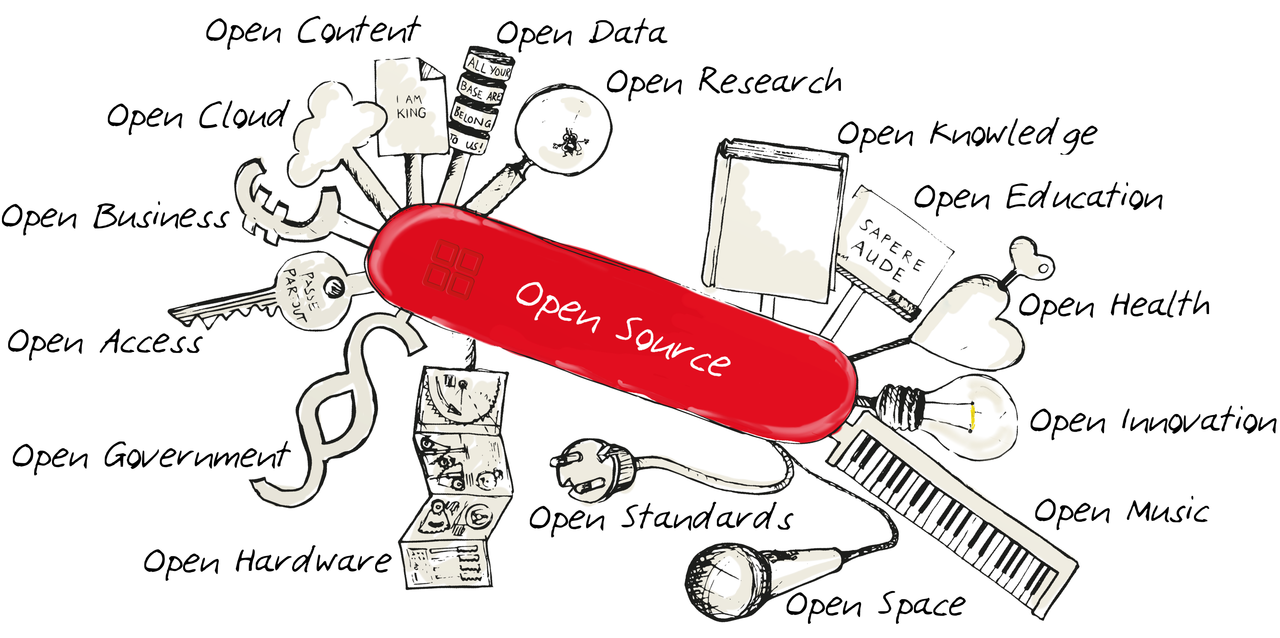
\includegraphics[width=\linewidth]{resources/open_swiss_knife.png}
		Die \textbf{F}ree and \textbf{O}pen \textbf{S}ource \textbf{S}oftware \textbf{AG} stellt sich vor... 
	\end{frame}

	\begin{frame}
		\frametitle{Fest im Programm}
			wöchentliches Treffen\\
			tba, OH 12 - 4.037
	\end{frame}

	\begin{frame}
		\frametitle{Andere Projekte}
		\begin{itemize}
			\item Linux-Installationspartys
			\item CTF in der O-Phase
			\item Vortragsreihen zu FOSS
			\item Stand beim Sommerfest
			\item Fahrten zu Chaos-Events
		\end{itemize}
	\end{frame}
	\begin{frame}
		\frametitle{Geplant für dieses Semester}

			
			\centering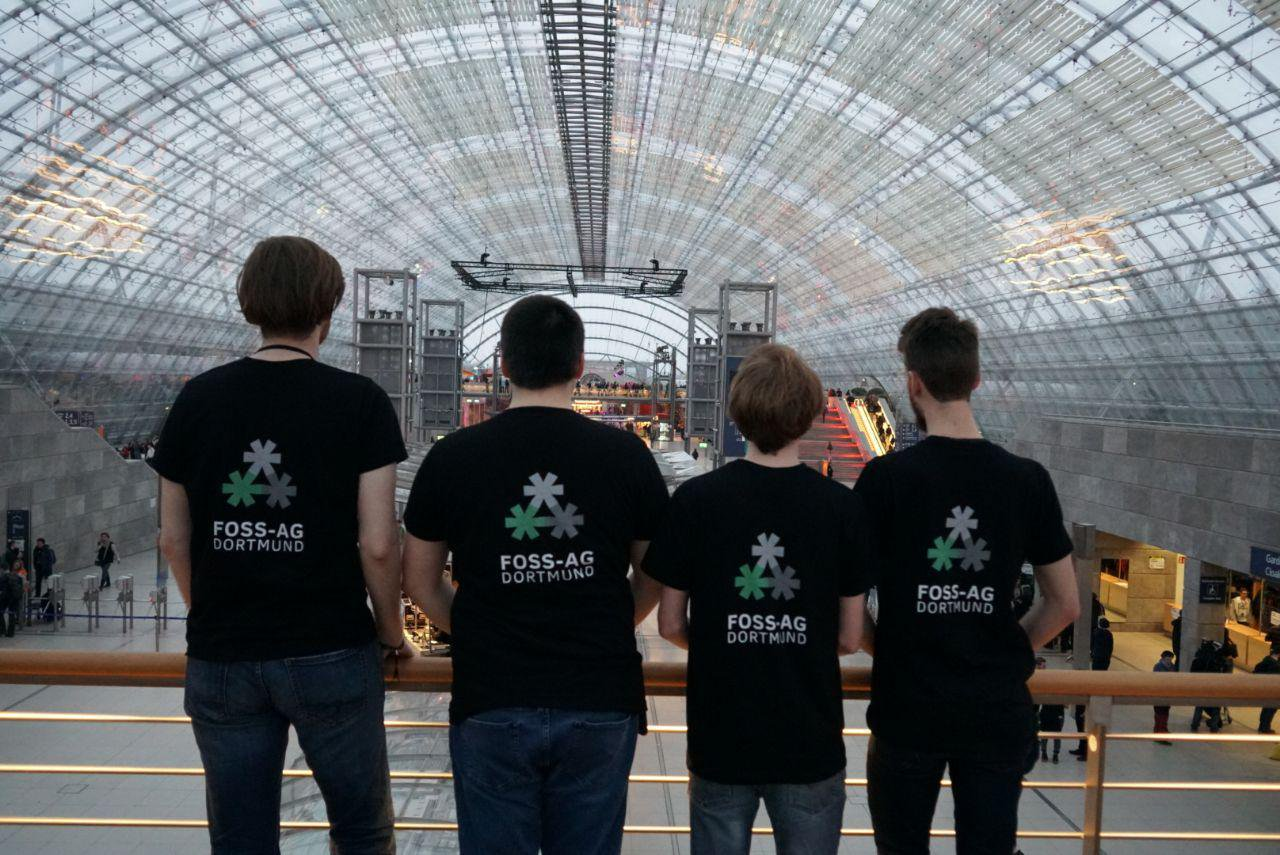
\includegraphics[width=0.9\linewidth]{resources/35C3.jpeg}
		\begin{itemize}
			\item Fahrt zum 36C3
			\item Hackathon
		\end{itemize}
	\end{frame}

	\begin{frame}
		\frametitle{Aktionen heute}
		\begin{itemize}
			\item Linux installieren
			\item Über FOSS unterhalten
			\item FOSS-AG CTF	
		\end{itemize}
	\textbf{Raum: E37 ab 15:00 Uhr}
	\end{frame}
	
	\begin{frame}
		\frametitle{Capture the Flag}
		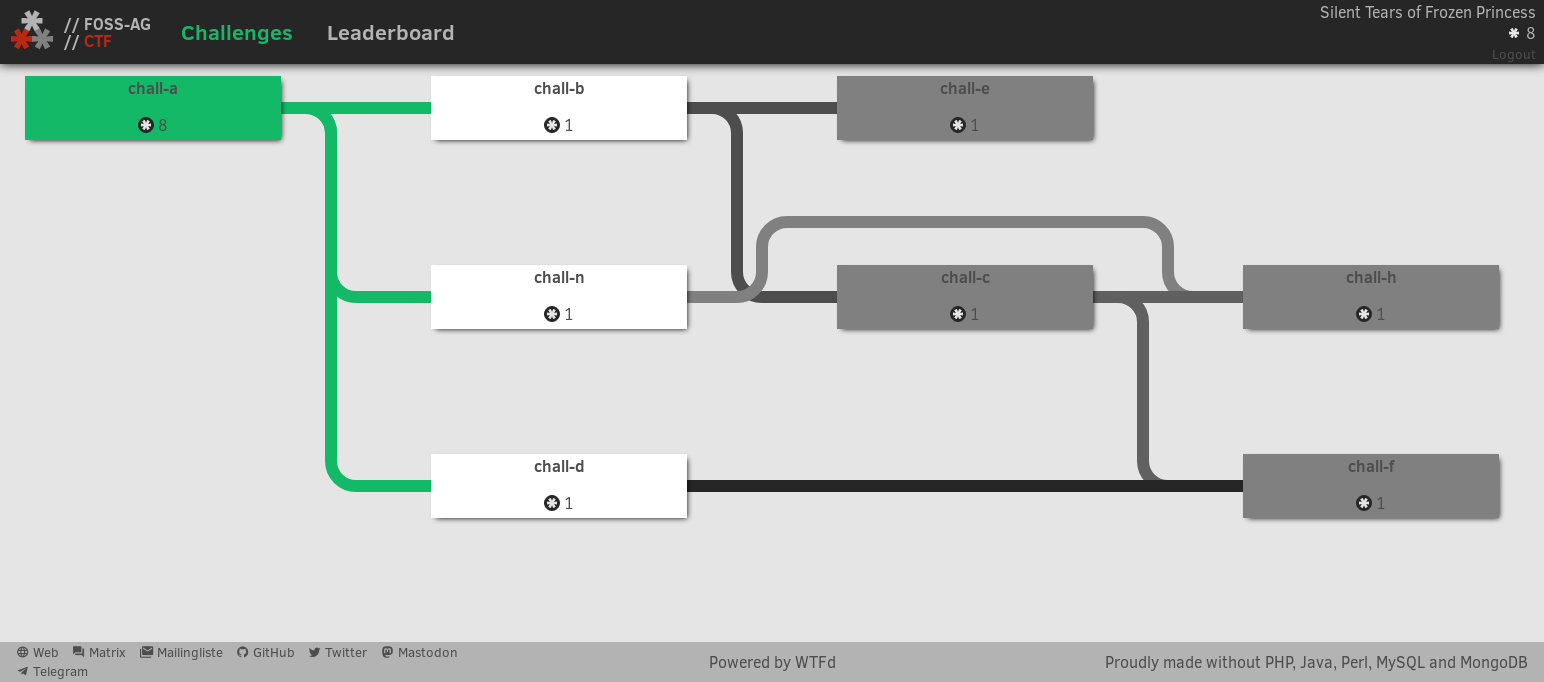
\includegraphics[width=\linewidth]{resources/screenshot_ctf.png}
		\begin{itemize}
			\item Rätsel in der Linuxwelt
			\item einige leichte, aber auch schwierigere
		\end{itemize}
	\end{frame}
	
	\begin{frame}
		\frametitle{Kontakt}
		\begin{itemize}
			\item \texttt{foss-ag.de}
			\item Matrix: \texttt{\#foss\_ag:fachschaften.org}
			\item Telegram-Channel: \texttt{@FOSSAG}
			\item Twitter: \texttt{@FOSSAGTUDO}	
			
		\end{itemize}
	\end{frame}

\end{document}
